\subsubsection{Data prefetch}
For the part of data prefetching EmporioLambda uses Next.js pre-rendering.\\
In fact Next.js allows the use 2 types of pre-rendering:
\begin{itemize}
\item static generation: generates the HTML at build time. The pre-rendered HTML is then reused on each request;
\begin{figure}[H]
\centering
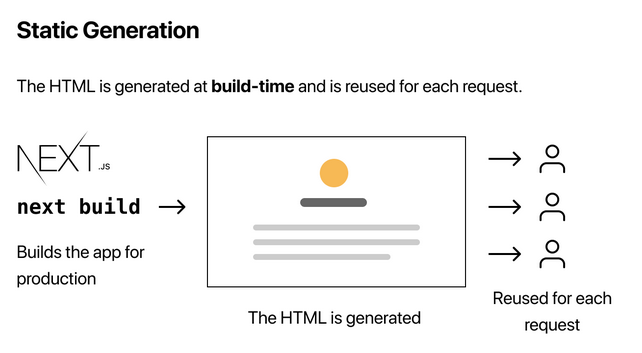
\includegraphics[scale=0.70]{res/Architettura/Frontend/img/staticGeneration}\\
\caption{Static generation scheme}
\end{figure}
\vspace{0.7cm}
\item server-side rendering: generates the HTML on each request.
\begin{figure}[H]
\centering
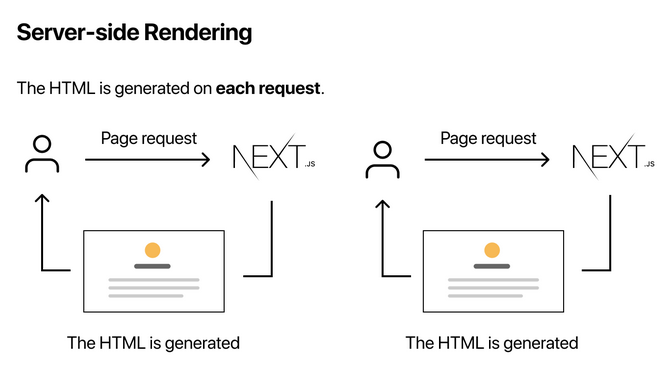
\includegraphics[scale=0.70]{res/Architettura/Frontend/img/serverSideRendering}\\
\caption{Static generation scheme}
\end{figure}
\vspace{0.7cm}
\end{itemize}
There's also a difference about the response time of the website with these 2 pre-rendering methods. Static generation is faster than server-side rendering so the second one should be used only when necessary. Each page can use a different type of prefetch.\\
In EmporioLambda each page prefetch data using these 2 methods:
\begin{itemize}
\item getStaticProps: this is a function, that return an object GetStaticProps, which indicates that the page will use static generation.
\item getServerSideProps: this is a function, that return an object GetServerSideProps, which indicates that the page will use server-side rendering, so it will render again after receiving new data.
\end{itemize}
Both functions returns a Typescript object called props with the data needed that will be passed to the component part of the Front-end module.\\
More informations about Next.js pre-rendering can be found in this page: \url{https://nextjs.org/learn/basics/data-fetching/two-forms}.\\
Actually all the pages in EmporioLambda uses server-side rendering.